%%============================================================================%%
\documentclass[a5paper]{ltjsarticle}
\usepackage[margin=15mm]{geometry}
\usepackage{amsmath}
\usepackage{ascmac} % for \itembox
\usepackage{amsfonts} % for \mathbb
\usepackage{graphicx}
%%============================================================================%%
\title{曲線加速の設計(書き途中)}
\author{Ryotaro Onuki (kerikun11+github@gmail.com)}
\date{\today}
\pagestyle{headings}
\setlength\fullwidth\textwidth % to fit header size
\allowdisplaybreaks
%%============================================================================%%
\begin{document}
\maketitle
%%============================================================================%%
\section{概要}
曲線加速の設計は次の2つの段階に分かれている.
実際の走行に使用するのは設計2である.
設計1は設計2の補助である.
\begin{itembox}[l]{設計1}
    \quad
    始点速度から終点速度までの,
    最大躍度,最大加速度の拘束を満たす速度軌道を設計する.
    \begin{itemize}
        \item 飽和: $j_{\max},~ a_{\max} \in \mathbb{R}_+$
        \item 速度: $v_\mathrm{start},~ v_\mathrm{end} \in \mathbb{R}$
        \item 出力: $j(t),~ a(t),~ v(t),~ x(t),~ \forall t \in \mathbb{R}$
    \end{itemize}
\end{itembox}
\begin{itembox}[l]{設計2}
    \quad
    始点速度から目標速度までの,
    最大躍度,最大加速度,最大速度,移動距離の拘束を満たす速度軌道を設計する.
    \begin{itemize}
        \item 飽和: $j_{\max},~ a_{\max},~ v_{\max} \in \mathbb{R}_+$
        \item 速度: $v_\mathrm{start},~ v_\mathrm{target} \in \mathbb{R}$
        \item 変位: $d \in \mathbb{R}$
        \item 初期値: $v_\mathrm{start},~ t_\mathrm{start} \in \mathbb{R}$
        \item 出力: $j(t),~ a(t),~ v(t),~ x(t),~ \forall t \in \mathbb{R}$
    \end{itemize}
\end{itembox}
%%============================================================================%%
\section{設計1:移動距離拘束なし}
はじめに,
走行位置には拘束を設けず,
与えらた始点速度と終点速度を滑らかにつなぐ速度軌道を設計する.
\begin{figure}[htbp]
    \centering
    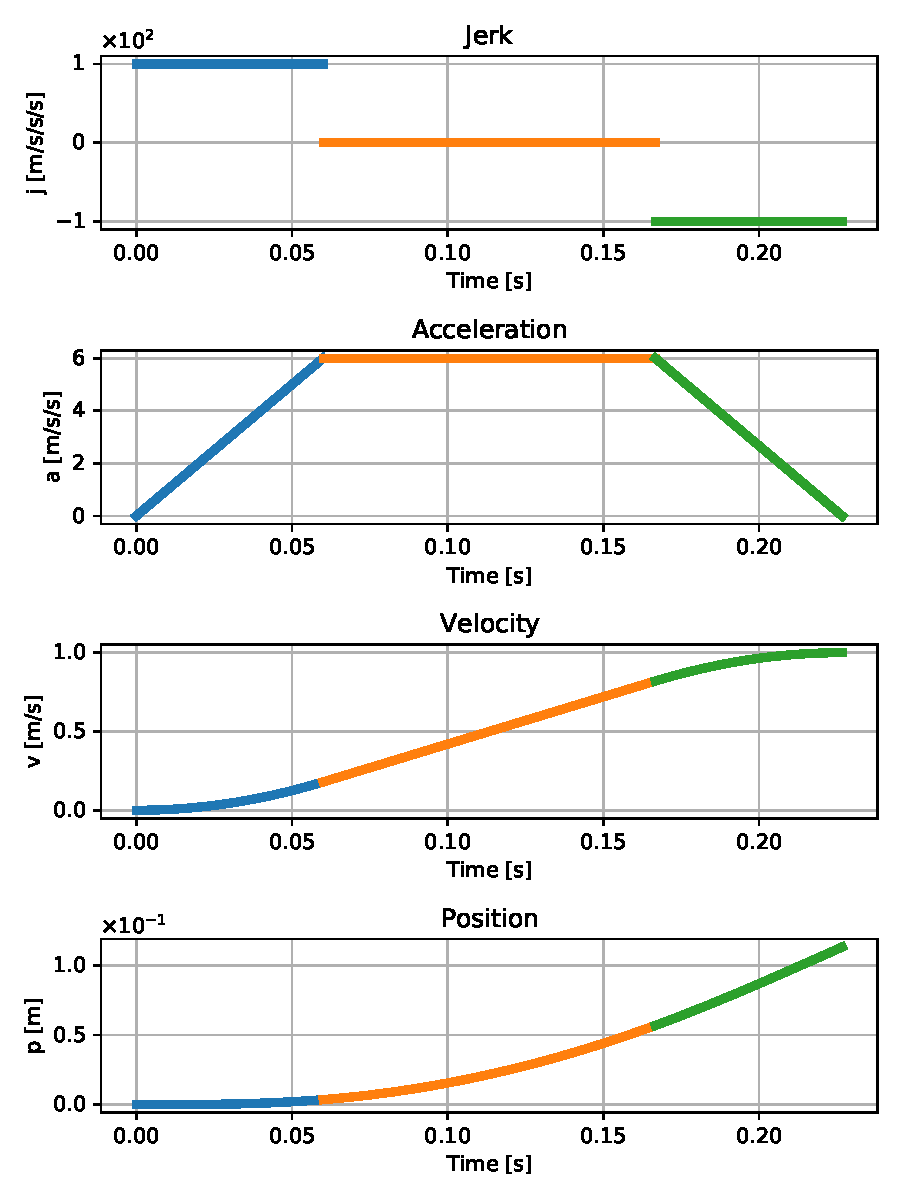
\includegraphics[width=0.8\linewidth]{figs/accel_curve.pdf}
    \caption{滑らかな速度軌道}
\end{figure}

\subsection{導出結果}
任意の時刻 $t$ における,躍度 $j(t)$, 加速度 $a(t)$, 速度 $v(t)$, 位置 $x(t)$
は,
\begin{align}
    j(t)
     & :=
    \left\{ \begin{array}{ll}
        0    & (\hspace{2.2em}t \le t_0) \\
        j_m  & (t_0 < t \le t_1)         \\
        0    & (t_1 < t \le t_2)         \\
        -j_m & (t_2 < t \le t_3)         \\
        0    & (t_3 < t \hspace{2.2em})
    \end{array} \right.
    \\
    a(t)
     & :=
    \left\{ \begin{array}{ll}
        0           & (\hspace{2.2em}t \le t_0) \\
        j_m(t-t_0)  & (t_0 < t \le t_1)         \\
        a_m         & (t_1 < t \le t_2)         \\
        -j_m(t-t_3) & (t_2 < t \le t_3)         \\
        0           & (t_3 < t \hspace{2.2em})
    \end{array} \right.
    \\
    v(t)
     & :=
    \left\{ \begin{array}{ll}
        v_0                           & (\hspace{2.2em} t \le t_0) \\
        v_0 + \frac{1}{2}j_m(t-t_0)^2 & (t_0 < t \le t_1)          \\
        v_1 + a_m(t-t_1)              & (t_1 < t \le t_2)          \\
        v_3 - \frac{1}{2}j_m(t-t_3)^2 & (t_2 < t \le t_3)          \\
        v_3                           & (t_3 < t \hspace{2.2em})
    \end{array} \right.
    \\
    x(t)
     & :=
    \left\{ \begin{array}{ll}
        x_0 + v_0(t-t_0)                           & (\hspace{2.2em} t \le t_0) \\
        x_0 + v_0(t-t_0) + \frac{1}{6}j_m(t-t_0)^3 & (t_0 < t \le t_1)          \\
        x_1 + v_1(t-t_1) + \frac{1}{2}a_m(t-t_1)^2 & (t_1 < t \le t_2)          \\
        x_3 + v_3(t-t_3) - \frac{1}{6}j_m(t-t_3)^3 & (t_2 < t \le t_3)          \\
        x_3 + v_3(t-t_3)                           & (t_3 < t \hspace{2.2em})
    \end{array} \right.
\end{align}
である.
ただし,
躍度定数 $j_m$,
加速度定数 $a_m$
\begin{align}
    j_m & = \mathrm{sign}(v_e-v_s) \times|j_{\max}| \\
    a_m & = \mathrm{sign}(v_e-v_s) \times|a_{\max}|
\end{align}
等加速度時間 $t_m$,
曲線速度時間$(t_m>0)$ $t_c$,
曲線速度時間$(t_m\leq 0)$ $t_c'$
\begin{align}
    t_m  & := \frac{1}{a_m}(v_e - v_s) - \frac{a_m}{j_m} \\
    t_c  & := \frac{a_m}{j_m}                            \\
    t_c' & := \sqrt{\frac{1}{j_m}(v_e-v_s)}
\end{align}
時刻定数 $t_0,~t_1,~t_2,~t_3$
\begin{align}
    \begin{array}{ll}
        \left\{ \begin{array}{l}
            t_0 := 0         \\
            t_1 := t_0 + t_c \\
            t_2 := t_1 + t_m \\
            t_3 := t_2 + t_c
        \end{array} \right.
         &
        (t_m > 0)
        \\
        \left\{ \begin{array}{l}
            t_0 := 0          \\
            t_1 := t_0 + t_c' \\
            t_2 := t_1        \\
            t_3 := t_2 + t_c'
        \end{array} \right.
         &
        (t_m \leq 0)
    \end{array}
\end{align}
速度定数 $v_0,~v_1,~v_2,~v_3$
\begin{align}
    \begin{array}{ll}
        \left\{ \begin{array}{l}
            v_0 := v_s                        \\
            v_1 := v_0 + \frac{1}{2}j_m t_c^2 \\
            v_2 := v_1 + a_m t_m              \\
            v_3 := v_e
        \end{array} \right.
         &
        (t_m > 0)
        \\
        \left\{ \begin{array}{l}
            v_0 := v_s                                     \\
            v_1 := v_0 + \frac{1}{2}\left( v_s+v_e \right) \\
            v_2 := v_1                                     \\
            v_3 := v_e
        \end{array} \right.
         &
        (t_m \leq 0)
    \end{array}
\end{align}
位置定数 $x_0,~x_1,~x_2,~x_3$
\begin{align}
    \begin{array}{ll}
        \left\{ \begin{array}{l}
            x_0 := 0                         \\
            x_1 := x_0 + v_0 t_c + j_m t_c^3 \\
            x_2 := x_1 + v_1 t_m             \\
            x_3 := x_0 + \frac{1}{2} (v_0+v_3) (2t_c+t_m)
        \end{array} \right.
         &
        (t_m > 0)
        \\
        \left\{ \begin{array}{l}
            x_0 := 0                                       \\
            x_1 := x_0 + v_1 t_c' + \frac{1}{6} j_m t_c'^3 \\
            x_2 := x_1                                     \\
            x_3 := x_0 + 2 v_1 t_c'
        \end{array} \right.
         &
        (t_m \leq 0)
    \end{array}
\end{align}
を定義する.

%%============================================================================%%
\subsection{設計手順}
前述の式を以下の手順で計算する.
\begin{enumerate}
    \item 躍度定数,加速度定数 $j_m,~a_m$ を求める.
    \item 時間定数 $t_m,~t_c,~t_c'$ を求める.
    \item 時刻定数 $t_i$ を求める.
    \item 速度定数 $v_i$ を求める.
    \item 位置定数 $x_i$ を求める.
    \item 関数 $j(t),~ a(t),~ v(t),~ x(t)$ を求める.
\end{enumerate}

%%============================================================================%%
\subsection{導出過程}
躍度の関数を適当に与えて,それを積分する形で導出した.

加速と減速の双方で共通の式を使用できるように,
躍度定数 $j_m \in \mathbb{R}$ および 加速度定数 $a_m \in \mathbb{R}$ を
\begin{align}
    j_m & = \mathrm{sign}(v_\mathrm{end}-v_\mathrm{start}) \times|j_{\max}| \\
    a_m & = \mathrm{sign}(v_\mathrm{end}-v_\mathrm{start}) \times|a_{\max}|
\end{align}
と定義する.

これらを用いて,
時刻 $t$ における,躍度 $j(t)$, 加速度 $a(t)$, 速度 $v(t)$, 位置 $x(t)$
\begin{align}
    j(t)
     & :=
    \left\{ \begin{array}{ll}
        0    & (\hspace{2.2em}t \le t_0) \\
        j_m  & (t_0 < t \le t_1)         \\
        0    & (t_1 < t \le t_2)         \\
        -j_m & (t_2 < t \le t_3)         \\
        0    & (t_3 < t \hspace{2.2em})
    \end{array} \right.
    \\
    a(t)
     & :=
    \left\{ \begin{array}{ll}
        0           & (\hspace{2.2em}t \le t_0) \\
        j_m(t-t_0)  & (t_0 < t \le t_1)         \\
        a_m         & (t_1 < t \le t_2)         \\
        -j_m(t-t_3) & (t_2 < t \le t_3)         \\
        0           & (t_3 < t \hspace{2.2em})
    \end{array} \right.
    \\
    v(t)
     & :=
    \left\{ \begin{array}{ll}
        v_0                           & (\hspace{2.2em} t \le t_0) \\
        v_0 + \frac{1}{2}j_m(t-t_0)^2 & (t_0 < t \le t_1)          \\
        v_1 + a_m(t-t_1)              & (t_1 < t \le t_2)          \\
        v_3 - \frac{1}{2}j_m(t-t_3)^2 & (t_2 < t \le t_3)          \\
        v_3                           & (t_3 < t \hspace{2.2em})
    \end{array} \right.
    \\
    x(t)
     & :=
    \left\{ \begin{array}{ll}
        x_0 + v_0(t-t_0)                           & (\hspace{2.2em} t \le t_0) \\
        x_0 + v_0(t-t_0) + \frac{1}{6}j_m(t-t_0)^3 & (t_0 < t \le t_1)          \\
        x_1 + v_1(t-t_1) + \frac{1}{2}a_m(t-t_1)^2 & (t_1 < t \le t_2)          \\
        x_3 + v_3(t-t_3) - \frac{1}{6}j_m(t-t_3)^3 & (t_2 < t \le t_3)          \\
        x_3 + v_3(t-t_3)                           & (t_3 < t \hspace{2.2em})
    \end{array} \right.
\end{align}
を考える.
ただし,$j(t)$を与えて順に積分を行った.
以下で各定数 $t_i,~ v_i,~ x_i$ を求める.

ここで,
加速中に等加速度直線運動が存在する場合と,存在しない場合があることに注意する.

曲線速度の時間 $t_c$ は,躍度 $j_m$ で加速度 $a_m$ になる時間なので,
\begin{align}
    t_c = \frac{a_m}{j_m}
\end{align}
と求めることができる.
次に,
等加速度直線運動の時間 $t_m$ を求める.
まず,
$v_s$ と $v_e$ の速度差が十分にあり, $t_m>0$ と仮定する.
加速度 $a(t)$ を各時刻区間において積分
\begin{align}
     &
    v_e
    =
    v_s + \int_{0}^{t_c}j_m t dt + \int_{t_c}^{t_c+t_m} a_m dt + \int_{t_c+t_m}^{t_c+t_m+t_c} (-j_m)(t-t_c-t_m) dt
    \\
     &
    \Leftrightarrow\quad
    t_m = \frac{1}{a_m}(v_e-v_s) - t_c
    = \frac{1}{a_m}(v_e-v_s) - \frac{a_m}{j_m}
\end{align}
をして,
等加速度直線運動の時間 $t_m$ を求めることができる.
したがって,
\begin{align}
    \begin{array}{ll}
        \left\{ \begin{array}{l}
            t_0 := 0         \\
            t_1 := t_0 + t_c \\
            t_2 := t_1 + t_m \\
            t_3 := t_2 + t_c
        \end{array} \right.
         &
        (t_m > 0)
        \\
        \left\{ \begin{array}{l}
            v_0 := v_s                        \\
            v_1 := v_0 + \frac{1}{2}j_m t_c^2 \\
            v_2 := v_1 + a_m t_m              \\
            v_3 := v_e
        \end{array} \right.
         &
        (t_m > 0)
        \\
        \left\{ \begin{array}{l}
            x_0 := 0                         \\
            x_1 := x_0 + v_0 t_c + j_m t_c^3 \\
            x_2 := x_1 + v_1 t_m             \\
            x_3 := x_0 + \frac{1}{2} (v_0+v_3) (2t_c+t_m)
        \end{array} \right.
         &
        (t_m > 0)
    \end{array}
\end{align}
が得られる.
ただし,
速度曲線の対称性より,走行距離 $x_3-x_0$ は,$x$軸と始点速度 $v_s$, 終点速度 $v_e$ からなる台形の面積に等しい.
したがって,
\begin{align}
    x_3-x_0 = \frac{1}{2}\left( v_e-v_s \right) \left( t_3-t_0 \right)
\end{align}
と求めることができる.

逆に, $t_m \leq 0$ となるとき,つまり,
最大躍度 $j_m$, 最大加速度 $a_m$, 始点速度 $v_s$, 終点速度 $v_e$ が
\begin{align}
     &
    t_m = \frac{1}{a_m}(v_e-v_s) - \frac{a_m}{j_m} < 0
    \\
     &
    \Leftrightarrow
    \quad
    \left\{
    \begin{array}{ll}
        v_e < v_s + \frac{a_m^2}{j_m} & (a_m \ge 0)
        \\
        v_e > v_s + \frac{a_m^2}{j_m} & (a_m <0)
    \end{array}
    \right.
\end{align}
の関係のとき,等加速度直線運動は存在しないことがわかる.
このとき,
新たな曲線加速の時間 $t_c',~(0 < t_c' < t_c)$ を求める.
始点速度 $v_s$ と 終点速度 $v_e$ および新たな曲線加速の時間 $t_c'$ の関係より,
\begin{align}
     &
    v_e = v_s + \int_{0}^{t_c'} j_m t dt + \int_{t_c'}^{t_c'+t_c'} (-j_m) (t-t_c') dt
    \\
     &
    \Leftrightarrow\quad
    t_c' = \sqrt{\frac{1}{j_m}(v_e-v_s)}
\end{align}
と求めることができる.
したがって,
\begin{align}
    \begin{array}{ll}
        \left\{ \begin{array}{l}
            t_0 := 0          \\
            t_1 := t_0 + t_c' \\
            t_2 := t_1        \\
            t_3 := t_2 + t_c'
        \end{array} \right.
         &
        (t_m \leq 0)
        \\
        \left\{ \begin{array}{l}
            v_0 := v_s                                     \\
            v_1 := v_0 + \frac{1}{2}\left( v_s+v_e \right) \\
            v_2 := v_1                                     \\
            v_3 := v_e
        \end{array} \right.
         &
        (t_m \leq 0)
        \\
        \left\{ \begin{array}{l}
            x_0 := 0                                       \\
            x_1 := x_0 + v_1 t_c' + \frac{1}{6} j_m t_c'^3 \\
            x_2 := x_1                                     \\
            x_3 := x_0 + 2 v_1 t_c'
        \end{array} \right.
         &
        (t_m \leq 0)
    \end{array}
\end{align}
が得られる.

\clearpage
%%============================================================================%%
\section{設計2:移動距離拘束つき}
つぎに,
走行距離の拘束を満たす滑らかな速度軌道を設計する.
実際に走行に使用する軌道である.
\begin{figure}[htbp]
    \centering
    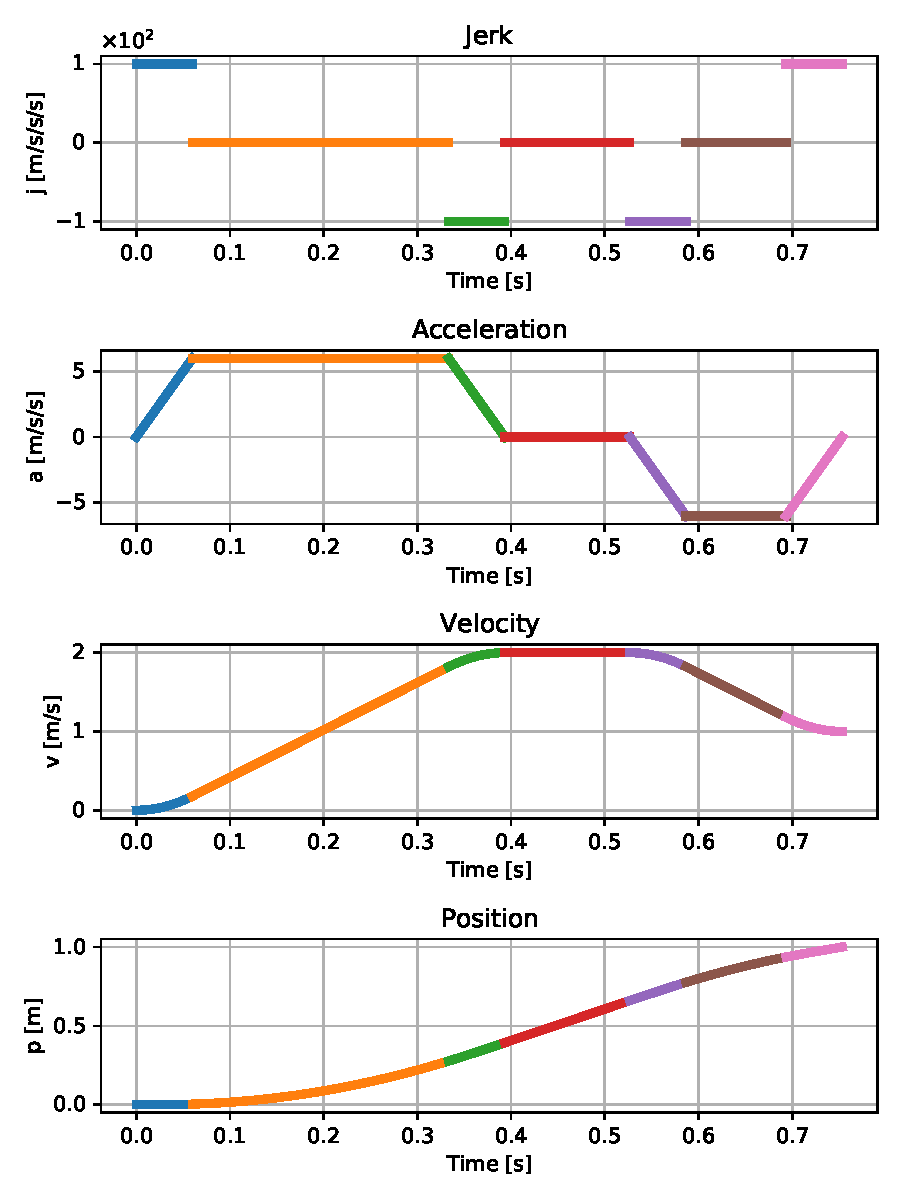
\includegraphics[width=0.8\linewidth]{figs/accel_designer.pdf}
    \caption{滑らかな速度軌道}
\end{figure}
\begin{table}[htbp]
    \centering
    \caption{変数のまとめ}
    \begin{tabular}{c|c|c|c|c}
        パラメータ & 記号  & 単位        & 属性   & 備考             \\ \hline\hline
        最大躍度   & $j_m$ & [m/s${}^3$] & 拘束   &                  \\
        最大加速度 & $a_m$ & [m/s${}^2$] & 拘束   &                  \\
        最大速度   & $v_m$ & [m/s]       & 拘束   &                  \\
        始点速度   & $v_s$ & [m/s]       & 初期値 &                  \\
        目標速度   & $v_t$ & [m/s]       & 目標値 & 目標終点速度     \\
        終点速度   & $v_e$ & [m/s]       & 結果   & 到達可能終点速度 \\
        移動距離   & $d$   & [m]         & 拘束   &                  \\
        始点時刻   & $t_s$ & [m]         & 初期値 & オプション       \\
        始点位置   & $x_s$ & [m]         & 初期値 & オプション       \\
    \end{tabular}
\end{table}

\subsection{導出結果}
始点速度 $v_s$ と目標速度 $v_t$ の速度差が小さいとき,
走行距離 $d$ の拘束により
目標速度 $v_t$ に達しない場合がある.
それを考慮して終点速度 $v_e$ を決定する.

終点速度 $v_e$
\begin{align}
    v_e(j_m,a_m,v_s,v_t,d) & :=
    \left\{
    \begin{array}{lll}
        v_t    & \mbox{if\quad}      & \|d\| \geq d_{v_s,v_t}
        \\
        v_{e1} & \mbox{else if\quad} & \|d\| \geq d_{t_m=0} \mbox{\quad and \quad} d\, v_{t_m=0} > 0
        \\
        v_{e2} & \mbox{else}
    \end{array}
    \right.
\end{align}
始点速度 $v_s$ から目標速度 $v_t$ まで変化するのに必要な最小移動距離 $d_{v_s,v_t}$
\begin{align}
    d_{v_s,v_t}(j_m,a_m,v_s,v_t) & := \frac{1}{2}(v_s+v_t) \, t_{v_s,v_t} \\
    t_{v_s,v_t}                  & :=
    \left\{\begin{array}{ll}
        2t_c + t_m & (t_m>0)    \\
        2t_c'      & (t_m\leq0)
    \end{array}\right.
\end{align}
等加速度が一定となる時間 $t_m$ ,
躍度が一定となる時間 $t_c,~t_c'$
\begin{align}
    t_m  & := \frac{1}{a_m}(v_t - v_s) - \frac{a_m}{j_m} \\
    t_c  & := \frac{a_m}{j_m}                            \\
    t_c' & := \sqrt{\frac{1}{j_m}(v_t-v_s)}
\end{align}
等加速度時間 $t_m = 0$となるときの移動距離 $d_{t_m=0}$ ,終点速度 $v_{t_m=0}$
\begin{align}
    d_{t_m=0} & := \left( v_s + \frac{1}{2}a_m t_c \right) t_c
    \\
    v_{t_m=0} & := \frac{j_m}{a_m} d - v_s
\end{align}
終点速度
\begin{align}
    v_{e1}  & := \frac{-a_m t_c + \sqrt{a_m^2 t_c^2-4(a_m t_c v_s - v_s^2 - 2a_m d)}}{2}
    \\
    v_{e2}  & := c +\bar{c} - \frac{1}{3} a = c + \frac{4a^2}{9c} - \frac{1}{3} a
    \\
    a       & := v_s
    \\
    b       & := j_m d^2
    \\
    c       & := \sqrt[3]{8a^3/27+b/2 + \|b\|\sqrt{8a^3/b/27+1/4}}
    \\
    \bar{c} & := \sqrt[3]{8a^3/27+b/2 - \|b\|\sqrt{8a^3/b/27+1/4}}
\end{align}
始点速度 $v_s$ と終点速度 $v_e$ ,移動変位 $d$ を満たす
到達可能速度 $v_r$
\begin{align}
    v_r := \frac{-a_mt_c \pm \sqrt{a_m^2t_c^2-(v_s+v_e)a_mt_c+4a_md+2(v_s^2+v_e^2)}}{2}
\end{align}
飽和速度
\begin{align}
    v_m = \min\{v_r,~v_{\max} \}
\end{align}
時刻定数を決定
\begin{align}
    \begin{array}{l@{~}l}
        t_0 & := t_0
        \\
        t_1 & := t_o + ac.t_{end}
        \\
        t_2 & := t_1 + \frac{d - ac.x_{end} - dc.x_{end}}{v_m}
        \\
        t_3 & := t_2 + dc.t_{end}
    \end{array}
\end{align}

\subsection{導出}

$$
    \begin{array}{l@{~}l}
        d_m & =                  \int_{t_0}^{t_1}v(t) dt + \int_{t_1}^{t_2}v(t) dt
        \\
            & =                  \int_{t_0}^{t_1}\left( v_0+\frac{1}{2} j_m(t-t_0)^2 \right) dt
        \\
            & \quad+ \int_{t_1}^{t_2}\left(
        v_0+                     \frac{1}{2} j_m(t_1-t_0)^2
        +j_m(t_1-t_0)(t-t_1) -   \frac{1}{2}j_m(t-t_1)^2
        \right) dt
        \\
            & = 2v_0t_c+a_mt_c^2
    \end{array}
$$

ただし,$j_m:=a_m/t_c$

$$
    \begin{array}{l@{~}l}
        d                      & = \frac{1}{2}(v_s+v_{e1})(t_3-t_0)
        \\
                               & = \frac{1}{2}(v_s+v_{e1})(t_c+t_m+t_c)
        \\
                               & = \frac{1}{2}(v_s+v_{e1})\left(t_c+\frac{v_{e1}-v_s}{a_m}\right)
        \\
        \Leftrightarrow v_{e1} & =
        \frac{1}{2}\left(\sqrt{4v_s^2-4v_sa_mt_c+a_m(a_mt_c^2+8d)}-a_mt_c\right)
    \end{array}
$$

$$
    \begin{array}{l@{~}l}
        d        & =                                                         \frac{1}{2}(v_s+v_{e2})(t_3-t_0)
        \\
                 & =                                                         \frac{1}{2}(v_s+v_{e2})2\sqrt{\frac{t_c}{a_m}(v_{e2}-v_s)}
        \\
        \Leftrightarrow
        v_{e2}^3 & + v_s v_{e2}^2-v_s^2v_{e2}-v_s^3-\frac{a_md^2}{t_c} = 0
        \\
        \Leftrightarrow
        v_{e2}   & =
        \frac{1}{3}\left(c +\frac{4a^2}{c}
        -a
        \right)
        \\
        a        & := v_s
        \\
        b        & :=                                                        \frac{a_md^2}{t_c}
        \\
        c        & :=                                                        \sqrt[3]{\frac{\sqrt{27b(32a^3+27b)} + 16a^3+27b}{2}}
    \end{array}
$$

以上をまとめると,たどり着き得る終点速度$v_{e1}$は,

$$
    v_{e} :=
    \left\{\begin{array}{ll}
        v_{e1} & (d        \ge d_m) \\
        v_{e2} & (d < d_m)
    \end{array}\right.
$$

始点速度 $v_s$ と終点速度 $v_e$ ,移動変位 $d$ を満たす
到達可能速度 $v_r$ の導出
\begin{align}
    d               & =
    \frac{1}{2}(v_s+v_r)(t_1-t_0)+
    \frac{1}{2}(v_r+v_e)(t_3-t_2)
    \\
                    & =
    \frac{1}{2}(v_s+v_r)\left(t_c+\frac{v_r-v_s}{a_m}\right)+
    \frac{1}{2}(v_r+v_e)\left(t_c+\frac{v_r-v_s}{a_m}\right)
    \\
    \Leftrightarrow & \quad
    v_r := \frac{-a_mt_c + \sqrt{a_m^2t_c^2-(v_s+v_e)a_mt_c+4a_md+2(v_s^2+v_e^2)}}{2}
\end{align}

$$
    v_m = \min\{v_r,~v_{\max} \}
$$

\end{document}
